\documentclass[%
    12pt,
    ngerman,
    fleqn,
    parskip=half,
    DIV=15, BCOR=2cm, headinclude,
]{scrbook}


\usepackage{cite}


\usepackage{header}

\def\table{\def\figurename{Tabelle}\figure}
\let\endtable\endfigure 

\usepackage{csquotes}
\usepackage{booktabs}
\usepackage{algpseudocode}
\usepackage{placeins}

\usepackage{caption}

\usepackage{diagbox}

\usepackage{pdfpages}


%\usepackage[backend=biber,style=alphabetic]{biblatex}
%\addbibresource{Quellen.bib}


\usepackage{float}
\newfloat{algorithm}{tbhp}{loa}[chapter]
\floatname{algorithm}{Algorithmus}

\usepackage{tikz}
\usepackage{pgfplots}


\hypersetup{
    pdftitle={%
        Konstruktion, Aufbau und Inbetriebnahme eines Wirbelbetts zur Granulatfluidisierung
    }
}

\usepackage{datetime}
\usepackage{wallpaper}


\newcommand\bootstrapsamples{N_\text P}
\newcommand\gausswidth{\sigma}
\newcommand\initialrandomwidth{\tilde \Delta}
\newcommand\iterations{M}
\newcommand\iterationsbetween{M_\text{Zw}}
\newcommand\margin{\Delta}
\newcommand\mass{\mu}
\newcommand\preiterations{M'}
\newcommand\rounds{\bar n}
\newcommand\timesites{N}
\newcommand\timestep{a}

%\addto\captionsngerman{\renewcommand{\bibname}{}}


\subject{
	FH Aachen \\
	Fachbereich Energietechnik \\
	Studiengang Physikingenieurwesen
	}
\title{%
    Konstruktion, Aufbau und Inbetriebnahme eines Wirbelbetts zur Granulatfluidisierung
}
\subtitle{Bachelorarbeit}
\author{
    Vorgelegt im Jahr 2016 von Christoph Hansen \\
    \small{geboren am 30. April 1992 in Aachen} \\
    Zum Erlangen des akademischen Grades \\    
    \large{Bachelor of Engineering (B.Eng.)}
    }
    
\date{}    

\publishers{%
	Angefertigt am Institut für Materialpyhsik im Weltraum am Deutschen Zenstrum für Luft- und Raumfahrt, vorgelegt dem Fachbereich 10 der Fachhochschule Aachen, Campus Jülich
	
	\begin{figure}[h]
		\begin{center}
				\includegraphics[scale=0.06]{DLR_Logo.png}
		\end{center}
	\end{figure}

}

\uppertitleback{%
    1. Prüfer: Prof. Dr.-Ing. Michael Stellberg \\
    2. Prüfer: Prof. Dr. Matthias Sperl 
}

\lowertitleback{%
	
	\small{
	Die vorliegende Arbeit ist bis zum 30.9.2017 streng vertraulich zu behandeln. Die Inhalte dieser Arbeit dürfen im oben genannten Zeitraum weder ganz, noch in Auszügen ohne Einwilligung der Firma Dritten zugänglich gemacht werden.
	Insbesondere darf die vorliegende Arbeit im genannten Zeitraum nicht in einer Bibliothek aufgestellt werden. Sie darf nur nach vorheriger Absprache mit Prof. Dr.-Ing. Michael Stellberg im Labor für Produktentwicklung der FH Aachen, Campus Jülich eingesehen werden.
	
	Die Weitergabe oder die Verwertung der Unterlagen, Informationen und/oder Kenntnissen ist ausnahmsweise zulässig, soweit dies zum ordnungsgemäßen Ablauf des Prüfungsverfahrens gemäß der Prüfungsordnung der FH Aachen erforderlich ist.
	}
	
	
	\vspace{2cm}
	
Ich versichere hiermit, dass ich die vorliegende Arbeit selbstständig verfasst und keine anderen als im Quellenverzeichnis angegebenen Quellen benutzt habe. Stellen, die wörtlich oder sinngemäß aus veröffentlichten oder noch nicht veröffentlichten Quellen entnommen sind, sind als solche kenntlich gemacht. Die Zeichnungen oder Abbildungen in dieser Arbeit sind von mir selbst erstellt worden oder mit einem entsprechenden Quellennachweis versehen. Diese Arbeit ist in gleicher oder ähnlicher Form noch bei keiner anderen Prüfungsbehörde eingereicht worden.
	
	\vspace{2cm}
	
	\hspace*{\fill}\begin{tabular}{@{}l@{}}\hline
		\makebox[6cm]{Christoph Hansen}
	\end{tabular}
	
	\vspace{2cm}
	
	Die Arbeit wurde betreut von: 
	
	\textcolor{white}{Das ist ein Platzhalter}

	\begin{minipage}{0.5\textwidth}
		\includegraphics[scale=0.6]{FH_Aachen_Logo.png}
	\end{minipage}
	\begin{minipage}{0.5\textwidth}
		Prof. Dr.-Ing. Michael Stellberg
	\end{minipage}
	\begin{minipage}{0.5\textwidth}
		\includegraphics[scale=0.04]{DLR_Logo.png}
	\end{minipage}
	\begin{minipage}{0.5\textwidth}
		Prof. Dr. Matthias Sperl
	\end{minipage}	
}




\begin{document}

%\maketitle

\includepdf[pages={1-5}, fitpaper=true]{FH_Aachen_Chris.pdf}

\CenterWallPaper{1}{Seitenhintergrund.png}

\cleardoublepage

\setcounter{page}{1}

\tableofcontents

\newpage

\chapter{Einleitung}

In der Einleitung wird eine Einführung in das Thema gegeben. Weiterhin werden die wichtigsten Definitionen erläutert und im weiteren die wissenschaftliche Fragestellung, die Ziele und die Arbeitsplanung näher erklärt.

\section{Einführung}

Diese Arbeit behandelt die Neukonzeption des bestehenden Wirbelbettes am Deutschen Zentrum für Luft- und Raumfahrt, Institut für Materialphysik im Weltraum. Ziel ist es das bestehende Wirbelbett zu einem Messaufbau weiterzuentwickeln um Wechselwirkungen in granularen Medien zu charakterisieren. Zur Verifikation der Konstruktion werden im Anschluss Testmessungen mit verschiedenen granularen Medien gemacht. \\
Im Folgenden werden grundlegenden Eigenschaften von Granulaten und Wirbelbetten behandelt. Danach werden die Anforderungen und Ziele erläutert, worauf die Beschreibung der Umsetzung folgt.


\section{Grundlegende Definitionen}

Im weiteren Verlauf wird zunächst erläutert, was granulare Medien physikalisch kennzeichnet und danach das Prinzip eines Wirbelbetts erläutert.

\subsection{Granulare Medien}

Unter Granulat versteht man ein Medium, das aus einzelnen harten Körnern besteht, die jeweils den Gesetzen der Newtonschen Mechanik unterworfen sind. Weiterhin haben die Körner eine Mindestgröße von $\SI{10}{\micro\meter}$, wodurch die thermische Anregung unterbunden wird. \\
Ein weiteres Charakteristikum von Granulaten ist die Dissipation. Das heißt, dass die hauptsächlich kinetische Energie der Körner durch Stöße fast komplett in Wärmeenergie umgewandelt werden kann. \cite{DLRWebsite} \\
Daraus ergibt sich als weiteres Merkmal granularer Medien die Segregation. Das bedeutet, das sich kleinere Partikel zwischen größeren bewegen können und so die Partikel nach Größen aufgetrennt werden. \cite{PhysikimKontext} \\
\hfill \\ 
Wie bei Molekülen gibt es auch bei granularen Medien ein dynamisches Verhalten. Dieses kann man unter anderem hervorrufen, indem man mittels Schwingungen, also Vibration, auf das Granulat einwirkt. Man erhält dann ein schwingungsfluidiertes Granulat, in dem die Bewegung der Teilchen mit der Brownschen Molekularbewegung vergleichbar ist. \\
Die unterschiedlichen dynamischen Zustände des Granulats werden gerne mit den Aggregatzuständen molekularer Stoffe verglichen:


\begin{center}
\begin{figure}[h]
	\includegraphics[scale=0.45]{Einleitung_1.jpg}
	\caption[Phasen im Wirbelbett]{Schema eines vertikal vibrationsangeregten Granulatbettes. Man sieht die unterschiedlichen Phasen, die ein Granulat je nach Vibrationsstärke annehmen kann. \cite{Darmstadt2015}}
\end{figure}	
\end{center}

Die in Abbildung 1.1 zu sehenden Phasen treten alle gleichzeitig während einer Anregung durch Vibration auf. Im gasförmigen Zustand sind die Abstände der Partikel weit größer als der Partikeldurchmesser und die Partikel bewegen sich weitgehend unabhängig voneinander. \\
Zum darunter liegenden flüssigen Zustand gibt es, anders als bei Wasser, keinen wohldefinierten Übergang. Man spricht von flüssig, sobald die mittlere freie Weglänge auf die Größenordnung der Partikel gesunken ist. Man spricht auch von einem Glasübergang. \\
Charakteristisch für granulare Medien ist der \glqq jamming\grqq-\ Übergang zwischen fest und flüssig. Hier ist keine Diffusion mehr möglich, die Partikel verbleiben also in ihrer Packungsposition und verklemmen mit ihrer Nachbarn. Bereits in diesem Zustand bilden sich sogenannte \glqq force chains\grqq \ heraus, über die die Kraftübertragung des Systems läuft. \\
Die \glqq force chains\grqq \ bilden sich im festen Zustand vollständig zu einem Netzwerk heraus. Da sich die Partikel amorph anordnen, verlaufen die \glqq force chains\grqq \ nicht homogen und isotrop, sondern willkürlich, was sich in einer unregelmäßigen Kraftverteilung ausdrückt \cite{Darmstadt2015, Fallturmexperiment}.
Eine genaue Charakterisierung der Wechselwirkung in einem granularen Medium mit der Methode von Castellanos möglich \cite{Castellanos2000}. Hierzu wird ein Wirbelbett genutzt, das im folgenden Abschnitt (1.2.2) erläutert wird. Diese Methode macht sich die Eigenschaft zunutze, das sich granulare Medien abhängig von den Wechselwirkungen der Teilchen untereinander und der Größe der Teilchen unterschiedlich verhalten und fluidisiert werden. Fluidisierung heißt in diesem Kontext, dass sich das granulare Medium wie eine Flüssigkeit verhält.

\subsection{Wirbelbett}

Um das Messprinzip von Castellanos zu nutzen und granulare Medien zu fluidisieren, soll folgender Aufbau verwendet werden.


\begin{figure}[h!]
		\begin{center}
		\includegraphics[scale=0.5]{Prinzip_Wirbelbett.png}
		\caption[Messaufbau Wirbelbett]{Schema des Messaufbau zur Charakterisierung von granularen Medien. Luft wird vom Massenstromregler entweder über den Luftbefeuchter oder direkt durch das Granulat geleitet. Dabei wird mit dem Drucksensor der über dem Granulat abfallende Druck gemessen}
	\end{center}
\end{figure}	


Das im Probenrohr befindliche granulare Medium wird von unten von einem durch einen Massenstromregler regelbaren Luftstrom durchströmt. Das Ziel ist hierbei, den Zustand der sogenannten \glqq Fluidisation\grqq \ zu erreichen. Um diesen Zustand messtechnisch zu bestimmen, ist es nötig, den über dem granularen Medium abfallenden Druck sehr genau zu messen. Das Ziel besteht darin, Graphen wie den unten stehenden zu erhalten:

\begin{figure}[h!]
	\begin{center}
		\includegraphics[scale=0.6]{Castellanos_Diagramm.jpg}
		\caption[Fluidisierungsdiagramm]{Druckdifferenz $\Delta p$ (Druck mit Granulat - Druck ohne Granulat) in Abhängigkeit vom Gasstrom. Der Breaking Point ist charakteristisch für das jeweilige Granulat und markiert den Übergang in den flüssigen Zustand \cite{Castellanos2000}}
	\end{center}
\end{figure}

Dabei muss besonders der zu sehende Peak (Breaking Point) gut vermessen sein, da sich über dessen Lage und Höhe die granularen Medien charakterisieren lassen. \\
Neben der Bestimmung mittels Druckabfall, lässt sich der Punkt der Fluidisation auch mittels Lichtstreuung bestimmen. Dazu wird das Ganulat mit einem Laser punktuell bestrahlt. Aus der Änderung des Streulichts lässt sich der Fluidisationspunkt bestimmen. 


\newpage

\section{Derzeitiger Stand und Probleme}


Das bisherige Wirbelbett besteht aus einem eingesteckten Röhrchen mit einem herkömmlichen Schwamm als Filter. Das Röhrchen und die Gaszufuhr sind beide auf einem hohlen Metallblock montiert. Mittels Kleber wird der luftdichte Abschluss erreicht. \\
Das oben beschriebene Teil ist zur vertikalen Verstellbarkeit auf einen Geräteträger montiert, für die horizontale Verstellbarkeit sorgt eine Mikrometerschraube auf dem Geräteträger. 

\begin{figure}[h!]
	\begin{center}
		\includegraphics[scale=0.3]{Altes_Wirbelbett_oben.png}
		\caption[Alter Aufbau 1]{Bestehender des Gassystems und der Elektronik.}
	\end{center}
\end{figure}	


Die Gaszufuhr wird über flexible Plasikschläuche realisiert, die teils mit Klemmen und teils mit Muttern an den Geräteflanschen befestigt sind. \\
Die Elektronik zum Auslesen des Drucksensors liegt offen und anfällig auf dem Tisch. Zudem kann der Druck noch nicht genau genug ausgelesen werden. Man bekommt ein Signal zwischen \SIrange{0}{10}{\volt} vom Sensor, das über einen Spannungsteiler auf \SIrange{0}{5}{\volt} reduziert wird. \\
Dieser Aufbau bringt eine Reihe von Problemen mit sich. Das größte Problem ist sicherlich, das nicht mit unterschiedlichen Probenrohrdurchmessern gemessen werden kann. Die sind nötig um auch große Partikel messen zu können. Außerdem ist der luftdichte Anschluss am Probenrohr nicht gegeben, da dies nur mit dem Schwamm in eine Öffnung des Metallblocks gesteckt wird.
Weiterhin ist das Wirbelbett zwar vertikal und horizontal beweglich, aber der Geräteträger verhindert Messungen im Lichtstreuaufbau.
Die bisherige Verrohrung mit Plastikschläuchen ist nicht luftdicht und zu instabil, um reproduzierbar messen zu können. \\


\begin{figure}[h!]
	\begin{center}
		\includegraphics[scale=0.6]{Kabel_Rohrleitungen_alt.png}
		\caption[Alter Aufbau 2]{Bestehende Rohrleitungen und Elektronik}
	\end{center}
\end{figure}


\section{Wissenschaftliche Fragestellung}

Es soll untersucht werden, ob die Wechselwirkung von Partikeln über Beschichtungen kontrolliert werden kann. Die Wechselwirkung soll über den Fluidisierungspunkt mit diesem Aufbau charakterisiert werden. Dazu muss eine große Bandbreite verschiedener Medien quantitaiv messbar sein. In diesem Fall bedeutet quantitativ vor allem, wie schon im vorigen Abschnitt \glqq Wirbelbett\grqq \ beschrieben, sehr hohe Präzision bei der Druckmessung. Dazu braucht man einen luftdichten Versuchsaufbau und einen ausreichend sensiblen Drucksensor. Physikalisch geht es dabei um um folgende Gleichungen: \\
Der Druckabfall über dem Granulat am Punkt der Fluidisation ist mit $\Delta P = \rho h g + \sigma_t$ gegeben. Hierbei ist $\rho$ die Dichte des Granulats und $\sigma_t$ der gemessene Peak aus Abbildung 1.3. Der Druckabfall ist außerdem mit der Carman-Gleichung $\Delta P / h = E \eta U \cdot \frac{1 - \epsilon}{\epsilon^3 d_p^2}$ gegeben. In diesem Fall ist $E$ eine Konstante mit Wert 180, $\eta$ die Gasviskosität, $U$ die Gasgeschwindigkeit, $d_p$ ist der Durchmesser des Probenröhrchens und $\epsilon$ die Porösität des Bettes. \\
Das Ziel der Arbeit ist die Realisierung eines Versuchsaufbau in dem die Strömungsgeschwindigkeit bzw. das Gasvolumen geregelt werden kann und der Druckabfall möglichst präzise vermessen werden kann.


\section{Ziele der Arbeit}

In der vorliegenden Arbeit soll ein vorhandener Versuchsstand für quantitative Messungen weiterentwickelt werden. Zuerst werden die Probleme des bisherigen Setups analysiert und eine entsprechende Lösung für das Medium Luft konstruiert. \\ 
Konkrete Ziele der Bachelorarbeit sind thematisch geordnet folgende:
Die Elektronik soll im Bezug auf das Auslesen des Drucksensors auf \SI{0,1}{mbar} genau sein und in ein Gehäuse verpackt werden. \\
Es soll ein neues Gassystem entworfen werden, das luftdicht und mechnanisch stabil ist. Weiterhin soll in das Gassystem ein Luftbefeuchter integriert werden. Außerdem sollen mit Probenröhrchen mit Durchmessern \SI{5}{mm}, \SI{20}{mm}, \SI{30}{mm} und \SI{40}{mm} gemessen werden. Die Röhrchen sollen einfach und schnell wechselbar sein und auch das Probenmaterial muss einfach zu wechseln sein. Um mit den größeren Röhrchendurchmessern $D_r$ und Partikeln $d_p$ messen zu können muss der Gasstrom erhöht werden. Aus den Gleichungen im vorigen Abschnitt ergeben sich, für die zwei häufigsten Packungsdichten ($\epsilon$), folgende Gasströme: 

Gasströme [l/h] für $\epsilon = \SI{0,54}{}$: \\

\begin{center}
	\begin{tabular}{|c|S|S|S|S|}
		\hline
		\diagbox{$D_r$ $[mm]$}{$d_p$ $[\mu m]$}    & 300   & 500   & 750   & 1000 \\
		\hline
		5     & 4,261 & 11,837 & 26,633 & 47,349 \\
		10    & 17,045 & 47,349 & 106,535 & 189,396 \\
		20    & 68,182 & 189,396 & 426,141 & 757,584 \\
		30    & 153,410 & 426,141 & 958,817 & 1704,564 \\
		40    & 272,730 & 757,584 & 1704,564 & 3030,336 \\
		\hline
	\end{tabular}
\end{center}


\vspace{1cm}

Gasströme [l/h] für $\epsilon = \SI{0,64}{}$: \\

\begin{center}
	\begin{tabular}{|c|S|S|S|S|}
		\hline
		\diagbox{$D_r$ $[mm]$}{$d_p$ $[\mu m]$}    & 300   & 500   & 750   & 1000 \\
		\hline
		5     & 12,831 & 35,643 & 80,197 & 142,573 \\
		10    & 51,326 & 142,573 & 320,789 & 570,292 \\
		20    & 205,305 & 570,292 & 1283,157 & 2281,169 \\
		30    & 461,936 & 1283,157 & 2887,105 &  5132,631 \\
		40    & 821,221 & 2281,169 & 5132,631 & 9124,678 \\
		\hline
	\end{tabular} 
\end{center}


\vspace{0.5cm}
Aus den Tabellen folgt, das mit einem Gasstrom von \SI{3000}{l/h} fast alle Paarungen abgedeckt werden können. Daher soll der Gasstrom auf diesen Wert erhöht werden. \\
Zur Unterbindung der Elektrostatik des granularen Mediums ist die Integration eines Luftionisators und Luftbefeuchters geplant. Weiterhin soll das Wirbelbett für eine korrekte Integration in den Lichtstreuaufbau horizontal und vertikal manipulierbar sein. \\
Zur Strukturierung der Arbeit wurden die einzelnen Ziele im folgenden Abschnitt unterteilt und ein Zeitplan aufgestellt.

\section{Arbeitsplanung}

Im Folgenden werden die einzelnen Arbeitspakete definiert und ein Überblick auf die zeitliche Einteilung der Abschnitte gegeben. 

\subsection{AP 1 - Analyse}

In diesem Arbeitspaket werden die Eckdaten des Projekts gesammelt und den Anforderungen zugeordnet. Zudem wird über die Materialwahl für das Wirbelbett entschieden und eine Stückliste aller Kaufteile für das Projekt erstellt. Außerdem werden erste Lösungsansätze definiert, was wiederum in die Liste der Kaufteile einfließt.


\subsection{AP 2 - Elektronik}

Aufgabe in diesem Arbeitspaket sind der Bau des Gehäuses und die Erhöhung der Präzision des Drucksensors. Dies soll zu Anfang geschehen, weil die Steuerelektronik für jegliche Steuerung zuständig ist und somit ohne diese das Wirbelbett nicht bedienbar ist. Zudem können mit einem recht einfachen Bauteil wie dem Gehäuse erste Erfahrungen mit dem 3D Drucker gesammelt werden.

\subsection{AP 3 - Gassystem}

Dieses Arbeitspaket beschäftigt sich mit dem Gassystem. Hier geht es insbesondere um das Suchen und Bestellen der geeigneten Teile für die Verrohrung und den Luftbefeuchter, sowie deren Zusammenbau. \\
Der Entschluss, dieses Arbeitspaket auch recht früh anzugehen fiel, auf Grund der langen Lieferzeit für den Flowcontroller. 

\subsection{AP 4 - Wirbelbett}

In diesem Arbeitspaket soll das eigentliche Wirbelbett neu konstruiert werden. Um schnell und effektiv beurteilen zu können, ob die Ideen zielführend sind, soll ein 3D Drucker zur Prototypenerzeugung genutzt werden. Die finalen Teile sollen ebenfalls mit dem 3D Drucker hergestellt werden. \\
Dieser Abschnitt liegt direkt vor dem Testen, damit unmittelbar nach dessen Abschluss alle für den Testlauf nötigen Komponenten vorhanden sind.


\subsection{AP 5 - Tests / Messungen}

Im letzten Abschnitt sollen alle Komponenten im vollständigen Aufbau getestet werden. Hier soll evaluiert werden, ob alle Anforderungen erfüllt wurden und ob es noch Mängel gibt. Kleinere Mängel sollen noch in dieser Phase behoben werden, während bei größeren analysiert werden muss, wie damit umzugehen ist. Wenn möglich werden auch Messkurven des alten Messaufbaus und des neuen verglichen und diskutiert.


\subsection{Zeitplanung}

Graphisch dargestellt stellt sich der Verlauf des Projekts so dar:

\begin{figure}[h]
	\begin{center}
		\includegraphics[scale=0.5]{Zeitplan_graphisch.jpg}
		\caption[Arbeitsplan]{Arbeitsplan für die einzelnen Arbeitspakete über die Bearbeitungszeit von 12 Wochen}
	\end{center}
\end{figure}



















\chapter{Praxisteil}

\section{AP 2 - Elektronik}

\subsection{Anforderungen}

Bei der Elektronik gab es zwei verschiedene Bereiche: \\
In einem ersten Schritt sollte ein A-D Wandler gefunden werden, damit der vorhandene Drucksensor genauer ausgelesen werden kann. Zum Start es Projekts wurde der Drucksensor über das $\SI{10}{bit}$ breite analoge Interface des Arduino ausgelesen. Das ist für eine genaue Auswertung der Experimente zu wenig. Der Drucksensor hat einen Messbereich von (nachgucken) und gibt diesen auf $\SI{0}{} - \SI{10}{V}$ aus. Da der Arduino maximal $\SI{5}{V}$ als Eingangsspannung verarbeiten kann, wird die Spannung über einen Spannungsteiler auf $\SI{0} - \SI{5}{V}$ reduziert und dann eingelesen. Das entspricht einer Genauigkeit von $\SI{0,004}{V/bit}$, was einer Genauigkeit von XXX mbar/Volt entspricht. \\
\hfill \\
Als Resultat soll die gesamte Elektronik als \glqq Blackbox\grqq \ vorliegen, sodass man nach außen hin nur noch Anschlüsse hat, die klar gekennzeichnet sind. Dies soll in Form eines Gehäuses erledigt werden, das zudem auch noch rudimentären Schutz gegen Schmutz bietet.


\subsection{Umsetzung}

\subsubsection{Elektronik}

Der Arduino bietet einen sehr einfachen SPI Bus zum Anschluss von Modulen an. Darüber können die digitalen Outputdaten, der angesteckten Module ausgelesen werden, unabhängig davon wie hoch die Auflösung der Module ist. Auf Grund dieser Voraussetzungen wurde entschieden ein Modul für diesen Bus zu verwenden. \\
Rechnung für 16 bit einfügen!!!!!! \\
Es gibt verschiedene $\SI{16}{bit}$ A-D Wandler auf dem Markt, allerdings gibt es den hier ausgewählten (einfügen!!!!) bereits auf einer fertig montierten Platine, die direkt in den Arduino eingesteckt werden kann. Zudem gibt es zu der Platine eine recht gute Dokumentation. 


Schaltskizze!!!

\subsubsection{Gehäuse}

Da es insbesondere im Lichtstreuaufbau nur sehr begrenzten Stauraum gibt und sämtliche Bauteile, das Wirbelbett selbst ausgenommen, auf einer Platte verbaut werden sollen, wurde gegen ein kommerziell erhältliches Gehäuse entschieden. \\ 
Stattdessen wurde ein Gehäuse entworfen, in dem sowohl der Arduino als auch das Board mit der Schaltung passgenau Platz finden. Dabei wurde darauf geachtet, dass die Kontakte unterhalb des Arduinos und des Boards genug Platz haben, sodass es keinerlei unbeabsichtigte Reibung der Komponenten am Gehäuse gibt. \\
Für die Anschlüsse wurden möglichst kleine Löcher im Gehäuse gelassen, sodass ein größtmöglicher Schutz gegen Schmutz bei größtmöglichem Komfort gewährleistet wird. \\
Um die Komplexität so gering wie möglich zu halten, wurde sich gegen einen Schließmechanismus entschieden, da dieser entweder anfällig oder unnötig teuer werden würde. Da das Gehäuse lediglich zum entfernen der angeschlossenen Kabel geöffnet werden muss, war es am einfachsten, den Deckel mit Klebeband am Gehäuse fest zu machen.

Hier Bilder einfügen!!


\section{AP3 - Gassystem}

\subsection{Anforderungen (kommt das hier hin?)}

Die Aufgabe bestand darin, trotz der Integration des Luftbefeuchters, das Gassystem als Einheit so kompakt und stabil wie möglich zu gestalten. Es sollte zusammen mit der Elektronik zusammen in den Lichtstreuaufbau passen und dort die Rotationbewegung des Aufbaus nicht einschränken.


\subsection{Umsetzung}

\subsubsection{Flowcontroller}

Um die Anforderung der Erweiterung des Regelbereichs beim Gasstrom auf $\SI{0} - \SI{3000}{l/h}$ zu erfüllen, musste der bisherige Flowcontroller mit einem Regelbereich von $\SI{0} - \SI{120}{l/h}$ ersetzt werden. \\
Die Idee einer konstruktiven Lösung den Strom über mehrere Gasdurchflussbegrenzer und Ventile auf definierte Werte voreinzustellen und mit dem vorhandenen Flowcontroller von da ab zu regeln, wurde verworfen, weil es sich als zu ungenau und nicht deutlich billiger in Aufwand und Kosten darstellte. \\
Die Lösung bestand darin einen neuen Flowcontroller anzuschaffen, der den gesamten Regelbereich mit einer hinreichenden Genauigkeit abdeckt und gleichzeitig gut in das Gassystem integriert werden kann. Dazu wurden Angebote eingeholt, die im folgenden dargelegt sind:

\begin{tabular}{|c|c|c|}
	\hline  & Brooks & Bronkhorst \\ 
	\hline Regelbereich & $\SI{0} - \SI{3000}{l/h}$ & $\SI{0} - \SI{3000}{l/h}$ \\ 
	\hline Genauigkeit $20 - \SI{100}{\%}$ & $\pm \SI{0,9}{\%}$ & $\pm \SI{0,5}{\%}$ Istwert $+ \pm \SI{0,1}{\%}$ Endwert\\ 
	\hline Genauigkeit $0 - \SI{20}{\%}$ & $\pm \SI{0,18}{\%}$ & $\pm \SI{0,5}{\%}$ Istwert $+ \pm \SI{0,1}{\%}$ Endwert \\ 
	\hline Preis in \euro & 1187,33 & 1382,66 \\ 
	\hline 
\end{tabular} 

\vspace{0,5cm}

Es wurde sich für den Flowcontroller der Firma Brooks entschieden. Das geschah aus mehreren Gründen: \\
Im ursprünglichen Aufbau war auch ein Flowcontroler von Brooks verbaut, daher wussten wir wie dieser angesteuert wird und hatten bereits den benötigten Stecker. Weiterhin ist die Genauigkeit des Brookscontrollers im niedriegen Regelbereich besser als die des Bronkhorstcontrollers. Dies ist grade bei quantitativen Messungen mit kleinen Rohrdurchmessern und sehr feinen granularen Medien essentiell. \\
Zudem waren die Anschaffungskosten für den Brookscontroller um ca $\SI{200}{Euro}$ niedriger.\\
Außerdem hatte die Gruppe bei einem anderen Controller von Bronkhorst einige Probleme mit der Zuverlässigkeit gehabt, während der Brooks Controller keine aufwies.


\subsubsection{Verrohrung}

Eine Herstellerauswahl hat hier nicht stattgefunden, da bereits vorhandene Verrohrung weitergenutzt werden sollte, deshalb wurde weiterhin auf Swagelok gesetzt. Dies hatte auch den Vorteil, das ein Berater aus dem nahegelegenen Standort Düsseldorf bei der Auslegung und Wahl der Komponenten beraten konnte. \\
Auf der Skizze in Abbildung xy kann man das gebaute System sehen:
\hfill \\

Skizze Einfügen


Bei der Verrohrung wurde sich für eine Kombination aus Edelstahlrohren und Bunaschläuchen entschieden. Dies bietet dem System die nötige Flexibilität im Bezug auf Anschluss an das Wirbelbett und die Luftzufuhr, als auch die nötige Robustheit und Stabilität. Sämtliche Rohrleitungen vom Druckminderer bis zum Übergang zum Wirbelbett sind aus Edelstahl. \\
Die Ventile, T-Stücke und Verbindungsstücke sind auch aus Edelstahl, da Messing zwar billiger wäre, allerdings auch weicher, was zu Verformungen und höherem Verschleiß führen kann.














\chapter{Bewertung und Ausblick}


\section{Bewertung}

In diesem Abschnitt soll der Erfolg der einzelnen Arbeitspakete kritisch hinterfragt werden, um Raum zur Optimierung aufzuzeigen. 

\subsection{Elektronik}

Rückblickend wurde der Arbeitsaufwand für die Elektronik unterschätzt, was dazu führte, dass sehr lange unklar war, welche Teile verwendet werden. Dadurch war es nicht möglich, in dem geplanten Zeitfenster ein finales Gehäuse für die Elektronik zu designen. Da bis zum Schluss keine finale Version der Elektronik vorlag, war es nicht möglich ein Gehäuse zu fertigen. In Zukunft wäre es besser, solche Probleme entweder früher zu erkennen oder das Design von vorne herein ans Ende zu stellen. 

\subsection{Gassystem}

Der gewählte Filter hat einen Nachteil. Trotz planem Aufkleben des Filters auf das Probenröhrchen, verformt sich dieser im Laufe der Nutzung plastisch. Das führt zu einem zusätzlichen Heben und Senken des granularen Mediums um bis zu \SI{2}{cm} (im Röhrchen mit \SI{30}{mm}  Durchmesser). Dieses Verhalten ist unerwünscht, da sich die Granulate deswegen nicht komprimieren und dann auf ihr Verhalten untersuchen lassen. Dieses Verhalten widerspricht allerdings nicht den ursprünglichen Anforderungen, die alle erfüllt wurden.

\subsection{Wirbelbett}

Die Konstruktion des Wirbelbettes erfüllt alle Anforderungen und verlief fast optimal. Lediglich gegen Ende musste, auf Grund der Umstellung von Kunststoff (ABS) auf Metall, die Konstruktion in einigen Punkten abgeändert werden. Das führte zu Zeitproblemen, da die Werkstatt zu dem Zeitpunkt ausgelastet war und nicht alle Röhrchenhalter rechtzeitig fertig wurden.
Im Vergleich mit der ursprünglichen Version wurde ein hochwertiges und quantitativ verwendbares Wirbelbett gebaut.

\subsection{Nutzung des 3D Druckers}

Durch die Anforderung, einen Ionisator im Aufbau unterzubringen, war es nicht möglich ein anderes Material außer Plastik zu verwenden. Zudem konnte eine andere Herangehensweise gewählt werden. Statt klassischen technischen Zeichnungen und FEM, wurde die Methode des evolutionären Druckens gewählt. Das sparte die aufwändigen Simulationen und erlaubte das Testen der designten Teile unter Realbedingungen. Der Nachteil dieser Methode ist neben den  Fehldrucken, die bei ca. \SI{10}{\%} lagen, der Ausschuss an Teilen. Dadurch, dass man dasselbe Teil in verschiedenen Evolutionsstufen druckt, ist der Materialverbrauch recht hoch. \\
Die Qualität der gedruckten Bauteile war durchweg hoch, besonders die Stabilität ist beachtlich. Allerdings sind zwei oder drei Drucke notwendig, bis man sein Modell am Rechner soweit angepasst hat, dass der Drucker so druckt, wie man es beabsichtigt. Zudem ist der Drucker anfällig in Bezug auf den Druckuntergrund. Während des Projekts ist das Kaptontape auf der Heizplatte kaputtgegangen. Ohne dieses Tape auf der Heizplatte, ist es nicht möglich Teile mit Durchmesser größer als \SI{40}{mm} mit flachem Boden zu drucken. Die Drucke bogen sich und waren somit ungeeignet, für dichtende Zwecke eingesetzt zu werden. Weiterhin stellte sich im Rahmen der Messungen heraus, dass der gedruckte Anschlusszylinder als auch der Röhrchenhalter nicht luftdicht ist. Die genauen Ursachen sind nicht untersucht worden, allerdings werden die nicht optimal miteinander verschmolzenen Außenwände dabei eine große Rollen spielen.
Ein Gruppenmitglied hat empfohlen das gedruckte Teil für knapp eine Minute in Aceton zu tauchen. Dabei wird die oberste Schicht des ABS aufgeschmolzen und versiegelt sich beim trocknen wieder. Das Ergebnis ist eine glasartige Oberfläche, die eine gute Luftdichtigkeit aufweisen könnte. 


\subsection{Zusammenfassung}

Abschließend kann gesagt werden, dass das Projekt sehr erfolgreich abgeschlossen wurde. Es wurden alle Anforderungen erfüllt und es ist nun möglich Granulate quantitativ zu vermessen.
Im Verlauf der Konstruktion wurden viele neue Erkenntnisse über das Verhalten verschiedener Tools und Materialien gewonnen. Dies sollte genutzt werden, um bei zukünftigen Projekten in diesem Bereich genauer planen und Risiken und Problemstellen besser einschätzen zu können.




\section{Ausblick}

Der Ausblick ist zweigeteilt. Im ersten Teil wird auf das konstruierte Wirbelbett eingegangen und im zweiten Teil über dessen Weiterentwicklung diskutiert. 

Wie bereits in der Bewertung erwähnt, gibt es noch Raum für Verbesserungen bei einzelnen Komponenten. Dies betrifft zum Beispiel den Filter, der entweder ersetzt werden sollte oder durch konstruktive Maßnahmen daran gehindert werden sollte, dass er sich biegen kann. In diesem Zusammenhang kann man sich auch nochmals mit der Integration eines Luftionisator beschäftigen, da dies ein interessantes Konzept ist- Unser Ionisator hatte allerdings entweder zu wenig Leistung hatte oder der Filter ließ zu wenig Ionen durch. \\
Weiterhin wäre es interessant zu untersuchen, ob und wie es möglich ist die 3D gedruckten Teile luftdicht zu machen. Eine Möglichkeit die erwogen wurde, ist das Tränken des gedruckten Teils in Epoxidharz. Bei einem Versuch mit Z-Bond 90 war die Behandlung nicht erfolgreich und der Luftduchfluss verschlechterte sich nocheinmal. Aceton hingegen schien vielversprechender zu sein. Hier wäre es interessant herauszufinden welche Materialien für eine luftdichte Versiegelung in Frage kommen und wie das gedruckte Teil damit behandelt werden muss. Der Vorteil wäre ein deutlich leichteres Wirbelbett.

Die Weiterentwicklung des Wirbelbetts bestünde darin, es auch mit Wasser betreiben zu können. Dies hat den Vorteil, dass durch den höheren Auftrieb des Granulats im Wasser und durch die höhere Viskosität des Wassers, deutlich weniger Strömungsmedium gebraucht wird. Im Gegensatz zu Luft mit bis zu \SI{3}{m^3/h}, würde es unter \SI{1}{l/h} Wasser benötigen, um die Teilchen zu fluidisieren. Zudem hat man bei der Verwendung von Wasser kein Problem mit Elektrostatik. \\
Der Nachteil von Wasser als Strömungsmedium besteht darin, das man eine Rückführung braucht und das Wasser im Kreislauf auch sauber gehalten werden muss. Zudem wäre eine neue Regelungstechnik für Wasser nötig, sowie ein neuer Drucksensor. Weiterhin führt die Verwendung von Wasser als Fluidisationsmedium zu einer geänderten Dynamik des Granulats und zu einer veränderten Wechselwirkung. Der Einfluss dessen auf die Messung ist bis jetzt unklar.  \\
Eine Umsetzung eines Wirbelbetts auf Wasserbasis wäre eine gute Folgebachelorarbeit.




\bibliography{Quellen}{}
\bibliographystyle{unsrt}

\addcontentsline{toc}{chapter}{Literaturverzeichnis}







\end{document}